%%%%%%%%%%%%%%%%%%%%%%%%%%%%%%%%%%%%%%%%%%%%%%%%%%%%%%%%%%%%%%%%%%%%%%%%%%%%%%%%
%% LaTeX Vorlage: ergebnisblatt_vorlage.tex                                   %%
%% Dies ist eine Vorlage fuer die Ergebissblaetter zu den Praktikumsaufagben  %%
%% der Vorlesung 'Einfuehrung in das Wissenschaftliche Rechnen'               %%
%%                                                                            %%
%% Version 2020-04-19, F. Castelli (IANM2, KIT)                               %%
%%%%%%%%%%%%%%%%%%%%%%%%%%%%%%%%%%%%%%%%%%%%%%%%%%%%%%%%%%%%%%%%%%%%%%%%%%%%%%%%
\documentclass[11pt,a4paper]{article}


%% Pakete
\usepackage[ngerman]{babel}
\usepackage[T1]{fontenc}
% \usepackage[utf8]{inputenc}   % Unix
\usepackage[latin1]{inputenc} % Windows
\usepackage[pdftex]{graphicx}
\usepackage{epstopdf}
\usepackage{amsmath,amssymb}

\DeclareMathAlphabet\mathbfcal{OMS}{cmsy}{b}{n}

%% Seitenlayout
\usepackage[DIV=12]{typearea}
\setlength{\parindent}{0em}


%% Font Helvetica
\renewcommand{\rmdefault}{phv}


%% Titelinformationen
\title{Einf\"uhrung in das Wissenschaftliche Rechnen\\
  Praktikumsblatt 3\\
  Aufgabe 5 (Von der Erde zum Mond)}
\author{Lena Hilpp Matr.Nr.: 1941997\\Jan Frithjof Fleischhammer Matr.Nr.: 2115491}
\date{13.05.2020}


%%%%%%%%%%%%%%%%%%%%%%%%%%%%%%%%%%%%%%%%%%%%%%%%%%%%%%%%%%%%%%%%%%%%%%%%%%%%%%%%
\begin{document}
  
  %% Titel
  \maketitle
  
  %%%%%%%%%%%%%%%%%%%%%%%%%%%%%%%%%%%%%%%%%%%%%%%%%%%%%%%%%%%%%%%%%%%%%%%%%%%%%%
  \section*{Problemstellung}
  %%%%%%%%%%%%%%%%%%%%%%%%%%%%%%%%%%%%%%%%%%%%%%%%%%%%%%%%%%%%%%%%%%%%%%%%%%%%%%
  In dieser Aufgabe wurde der Flug einer Rakete von der Erde zum Mond nach \textit{Jules Verne} modelliert und numerisch berechnet.\\
  
  Dabei wird die Rakete mit einer Anfangsgeschwindigkeit $v_0$ zum Zeitpunkt $t=0$ mit dem Abschusswinkel $\theta$ von der Erdoberfl\"ache abgeschossen. Dabei wird nur das Gravitationsfeld der Erde und des Mondes beachtet.\\
  Mit dem \textit{zweiten Newtonschen Gesetz} ($\mathbf{F}=m \mathbf{a}$) ergibt sich eine gew\"ohnliche Differenzialgleichung zweiter Ordnung f\"ur die Bewegung der Rakete.\\
  Da die Bewegung in einer Ebene stattfindet, kann man durch Rechnen in zwei Dimensionen Rechenaufwand sparen.\\
  
  Dabei beschreibt
  \begin{align*}
  V(x)=-\gamma(\frac{m_E}{dist_E(x)}+\frac{m_M}{dist_M(x)})
\end{align*}    
 das Gravitationspotential der Erde und des Mondes. $dist_E(\cdot)$ bzw. $dist_M(\cdot)$ ist dabei der Abstand zum Erdmittelpunkt bzw. Mondmittelpunkt.\\
 
 Die Gravitationsfeldst\"arke ist dann definiert durch
 \begin{align*}
 \mathbfcal{G}(x)=-\nabla V(x)
 \end{align*}
Daraus ergibt sich das Anfangswertproblem: Finde $\mathbf{x}:\mathbb{R}\to{\mathbb{R}}^2$, sodass
\begin{equation}
\begin{cases}
\mathbf{x}'' = \mathbfcal{G}(\mathbf{x}), \\
\mathbf{x}(\mathbf{0}) = \mathbf{x_0}, \\
\mathbf{v}(\mathbf{0}) = \mathbf{v_0}, \\

\end{cases}
\end{equation}
mit der Startposition $\mathbf{x_0}=[R_E,0]$ auf der Erdoberfl\"ache und der Abschussgeschwindigkeit $\mathbf{v_0}=v_0[cos(\theta),sin(\theta)]$.


  
  %%%%%%%%%%%%%%%%%%%%%%%%%%%%%%%%%%%%%%%%%%%%%%%%%%%%%%%%%%%%%%%%%%%%%%%%%%%%%%
  \section*{Ergebnis}
  %%%%%%%%%%%%%%%%%%%%%%%%%%%%%%%%%%%%%%%%%%%%%%%%%%%%%%%%%%%%%%%%%%%%%%%%%%%%%%
  
  In \textit{Abbildung 1} sind die Verl\"aufe des Gravitationspotentials und der Gravitationsfeldst\"arke aufgezeichnet. Dabei wurden die Raumkoordinaten entdimensioniert mit dem Referenzwert $x_{ref}=3.844\times10^8 m$, was dem Abstand von der Erde zum Mond entspricht. Somit liegt die Erde im Ursprung und der Mond in $(1,0)$.\\
  
  In \textit{Abbildung 2} ist der Verlauf der numerischen L\"osung, der zeitliche Verlauf der x-Koordinate, der Geschwindigkeit in x-Richtung sowie des Abstands zur Erde aufgetragen.\\
  
  Die Rakete ist dabei nach $6.6466$ Tage wieder auf der Erde.\\
  
    In diesem Model hat die Rakete einen Minimalabstand zur Mondoberfl\"ache von\\ $-9.404551\times10^5 m$, kollidiert also mit der Mondoberfl\"ache.\\
  
  In \textit{Abbildung 3} sieht man der Verlauf des Gravitationspotential der Rakete.\\
  
  Verwendet wurde dabei der \textit{matlab}-L\"oser \textit{ode45}, mit \textit{ode15s} und \textit{ode23s} erh\"alt man \"Ahnliche Ergebnisse.
  
  \begin{figure}
\begin{tabular}{cc}
  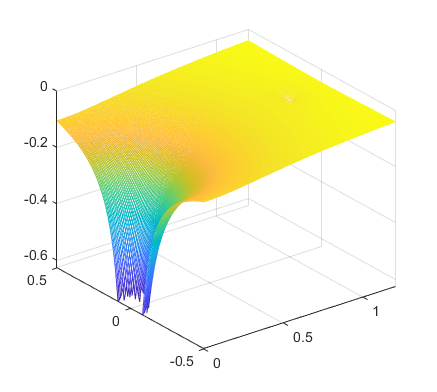
\includegraphics[width=0.45\textwidth]{bild1} &  
  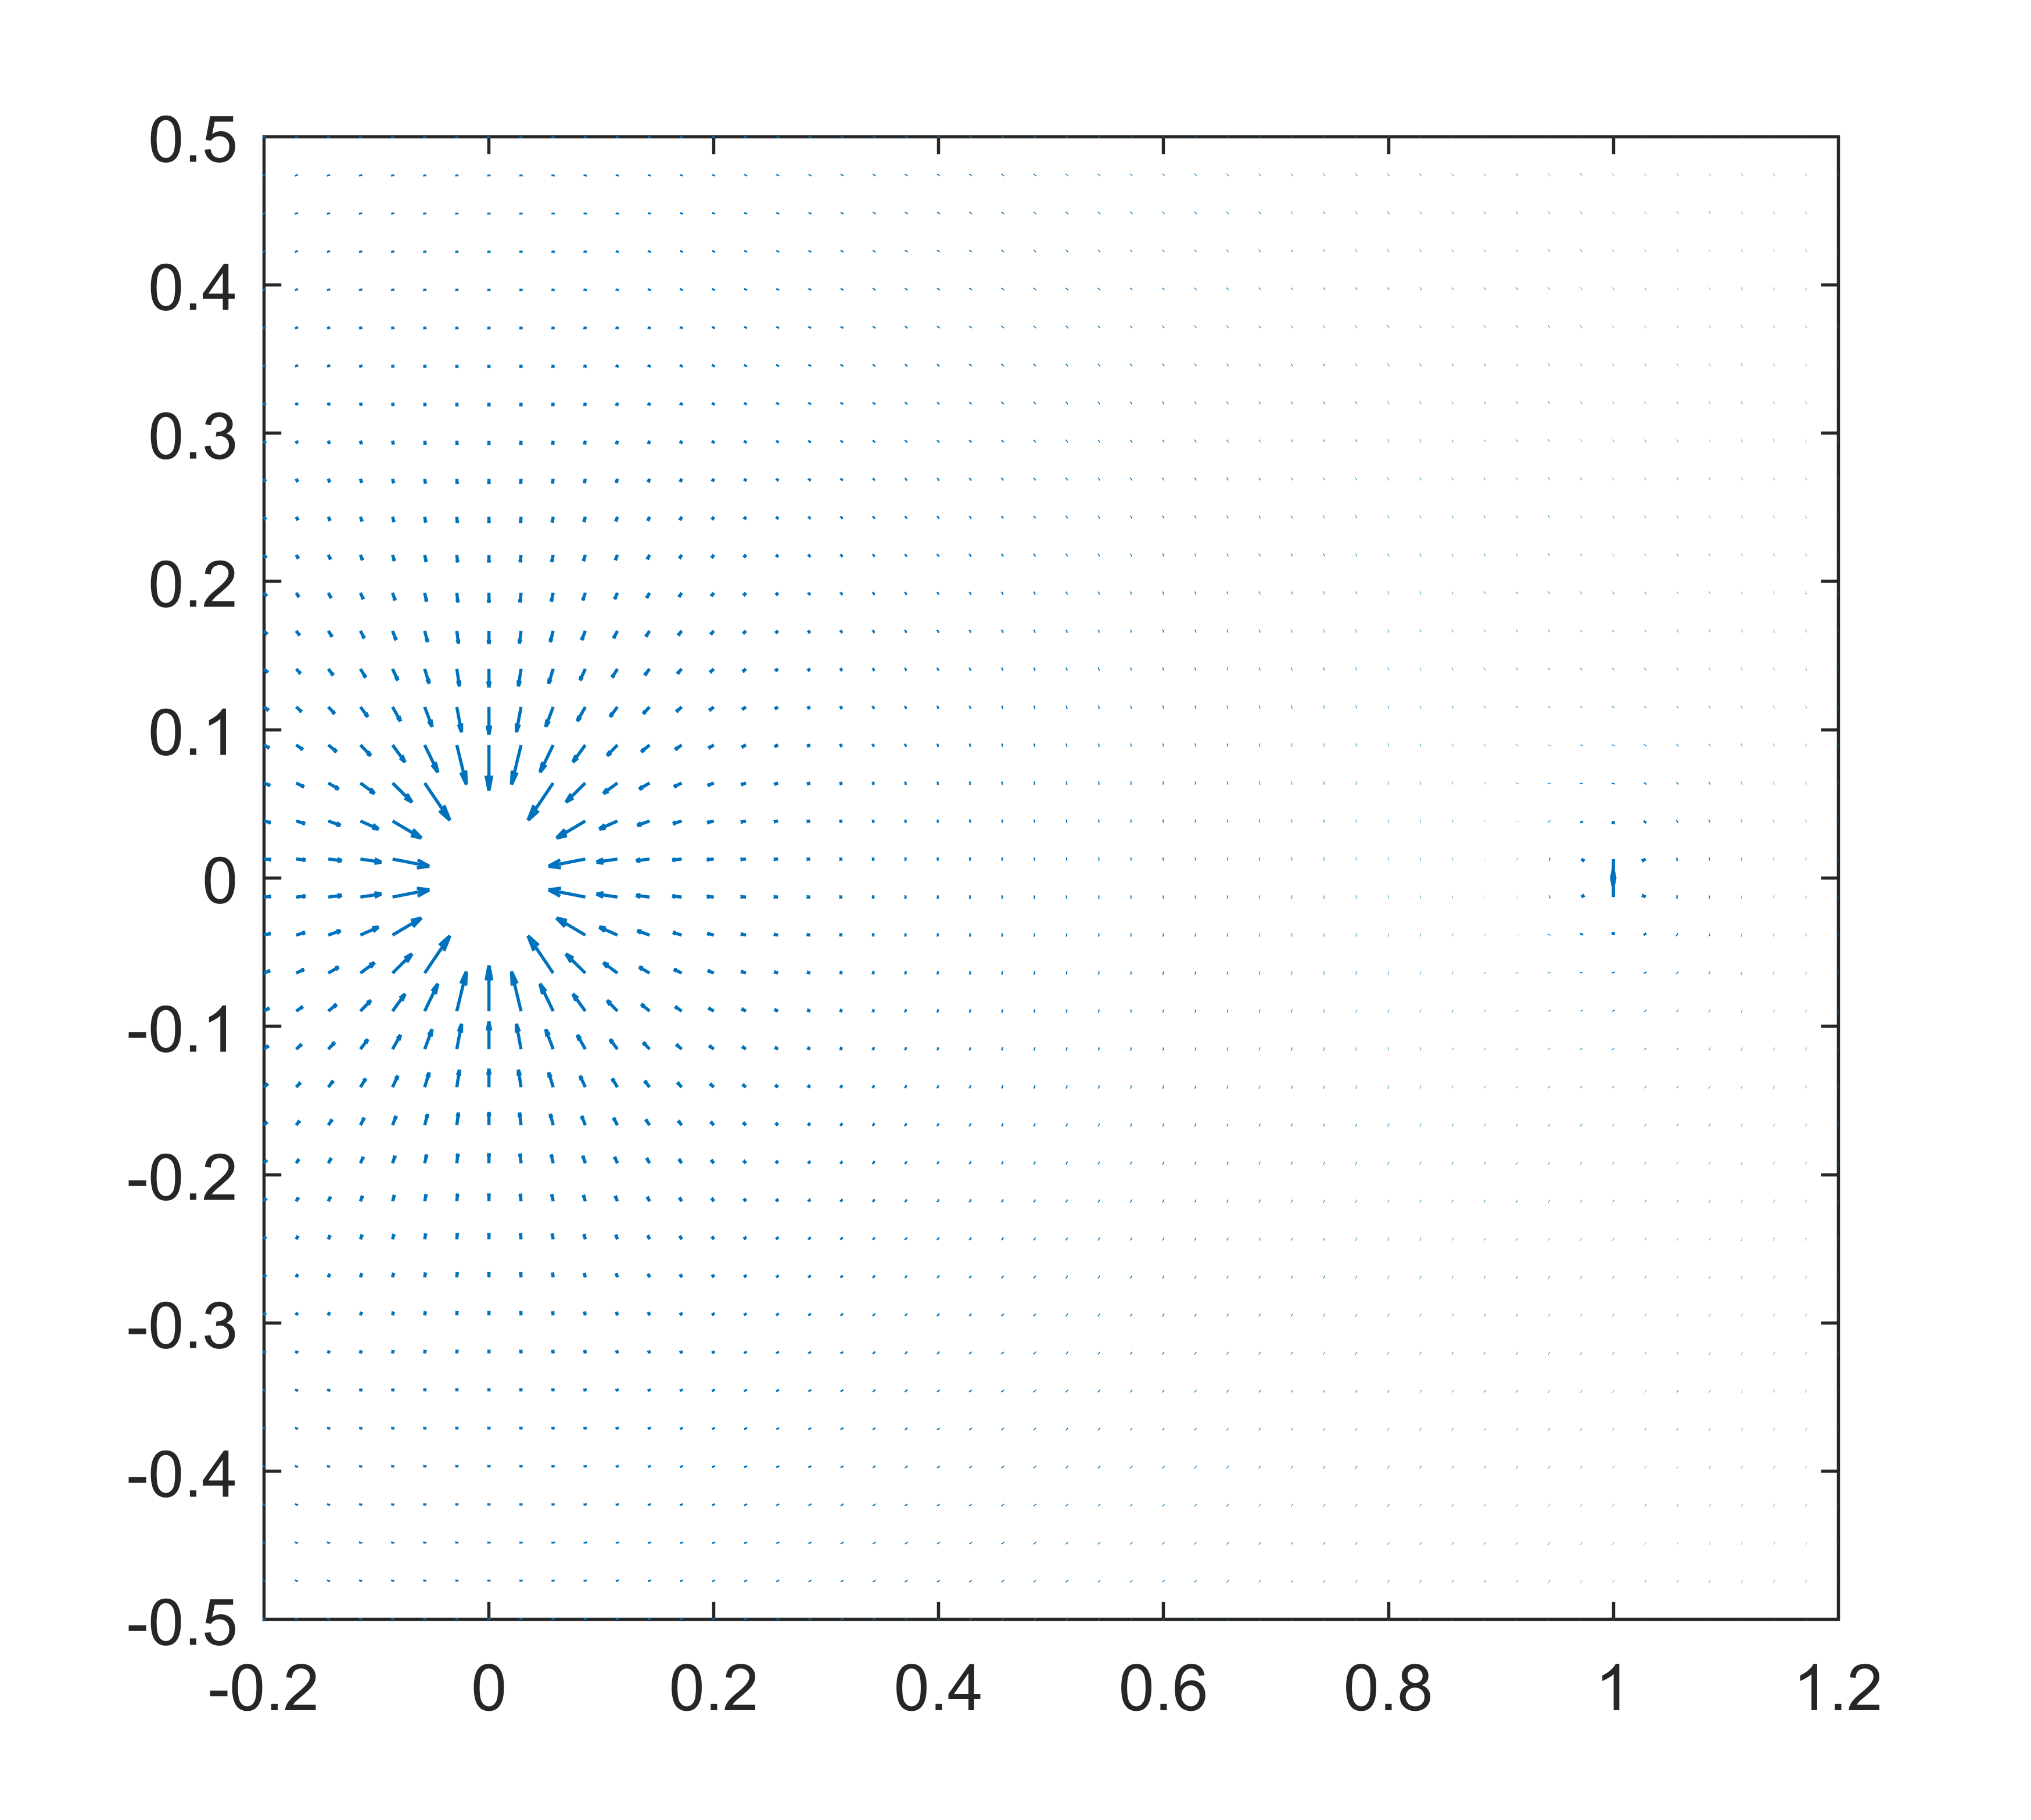
\includegraphics[width=0.45\textwidth]{bild2} \\
  
  \end{tabular}
\caption{Verlauf des Gravitationspotential (links) und der Gravitationsfeldst\"arke (rechts)}
  \end{figure}
  

\begin{figure}
\begin{tabular}{cc}
  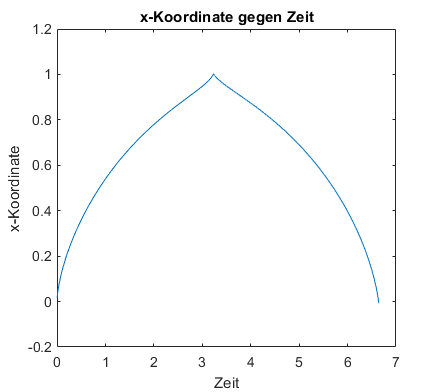
\includegraphics[width=0.45\textwidth]{bild4} &  
  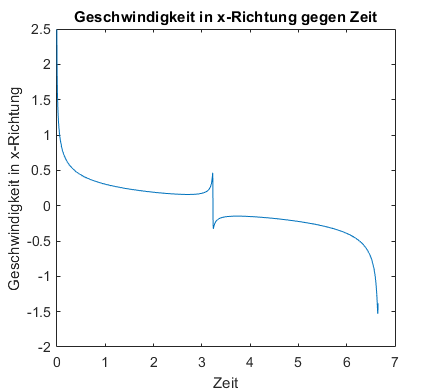
\includegraphics[width=0.45\textwidth]{bild5} \\
  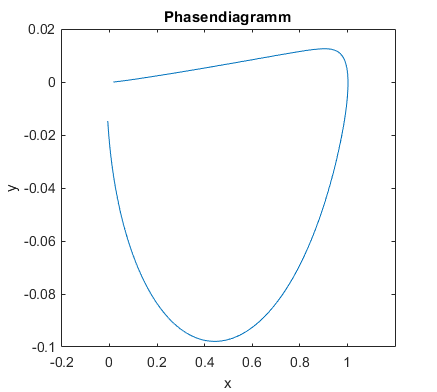
\includegraphics[width=0.45\textwidth]{bild6} &  
  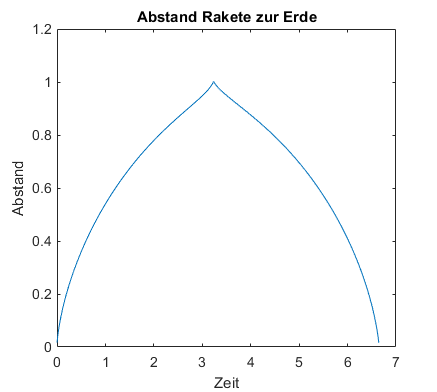
\includegraphics[width=0.45\textwidth]{bild7} \\
  
  \end{tabular}
\caption{Verlauf der numerischen L\"osung}
  \end{figure}
  
  \begin{figure}
  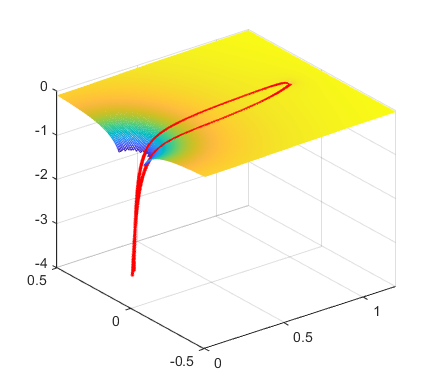
\includegraphics[width=0.5\textwidth]{bild8}
  \caption{Gravitationspotential der Rakete}
  \end{figure}
  
\end{document}
